\section{Физически изменяемые структуры данных}

Значения следующих типов: массивы, строки, записи с модифицируемыми полями и
указатели есть структурированные значения, компоненты которых могут быть
физически изменены.

Мы уже видели, что переменная в Objective CAML привязана к значению и хранит эту
связку до конца её существования. Мы можем изменить связку лишь
переопределением, но и в этом случае речь не будет идти о той же самой
переменной. Новая переменная с тем же именем скроет предыдущую, которая
перестанет быть доступной напрямую и останется неизменной. В случае с
изменяемыми переменными, мы можем ассоциировать новое значение переменной без её
переопределения. Значение переменной доступно в режиме чтение/запись.

\subsection{Векторы}

Векторы или одномерные массивы группируют определённое число однотипных
элементов. Существует несколько способов создания векторов, первый —
перечисление элементов, разделённых запятой и заключённых между символами [| и
|] .

\begin{lstlisting}[language=OCaml]
# let v = [| 3.14; 6.28; 9.42 |] ;;
val v : float array = [|3.14; 6.28; 9.42|]
\end{lstlisting}

Функция \texttt{Array.create} с двумя аргументами на входе: размер вектора и
начальное значение, возвращает новый вектор.

\begin{lstlisting}[language=OCaml]
# let v = Array.create 3 3.14;;
val v : float array = [|3.14; 3.14; 3.14|]
\end{lstlisting}

Для того чтобы изменить или просто просмотреть значение элемента необходимо
указать его номер.

Синтаксис

\begin{lstlisting}[language=OCaml]
expr1 . ( expr2 )
\end{lstlisting}

Синтаксис

\begin{lstlisting}[language=OCaml]
expr1 . ( expr2 ) <- expr3
\end{lstlisting}

\texttt{expr1} должен быть вектором (тип \texttt{array}) с элементами типа
\texttt{expr3}. Конечно, выражение \texttt{expr2} должно быть типа \texttt{int}.
Результат модификации есть выражение типа \texttt{unit}. Номер первого элемента
вектора 0 и последнего --- размер вектора минус 1. Скобки вокруг выражения
обязательны.


\begin{lstlisting}[language=OCaml]
# v.(1) ;;
- : float = 3.14
# v.(0) <- 100.0 ;;
- : unit = ()
# v ;;
- : float array = [|100.; 3.14; 3.14|]
\end{lstlisting}

Если индекс элемента не принадлежит интервалу индексов вектора, то возбуждается
исключения в момент доступа.

\begin{lstlisting}[language=OCaml]
# v.(-1) +. 4.0;;
Exception: Invalid_argument "index out of bounds".
\end{lstlisting}

Эта проверка осуществляется в момент выполнения программы, что может сказаться
на её быстроте. Однако, это необходимо для избежания заполнения зоны памяти вне
вектора, что может привести к серьёзным ошибкам.

Функции манипуляции векторами являются частью модуля \texttt{Array} стандартной
библиотеки, описание которого дано в главе \ref{??}. В следующих примерах мы
воспользуемся тремя функциями из этого модуля:

\begin{itemize}
	\item create создающая вектор заданного размера и начальным значением

	\item возвращающая размер вектора

	\item для конкатенации двух векторов 
\end{itemize}

\subsubsection{Совместное использование значений вектора}

 Все элементы вектора содержат значение, переданное во время создания вектора. В
случае, если это значение структурное, оно будет совместно использоваться
(sharing). Создадим, для примера, матрицу как вектор векторов при помощи функции
\texttt{Array.create}:

\begin{lstlisting}[language=OCaml]
# let v = Array.create 3 0;;
val v : int array = [|0; 0; 0|]
# let m = Array.create 3 v;;
val m : int array array = [|[|0; 0; 0|]; [|0; 0; 0|]; [|0; 0; 0|]|]
\end{lstlisting}

\begin{figure}[h]
	\center{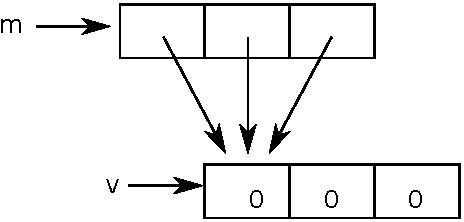
\includegraphics[width=\textwidth]
{img/memory_representation_of_a_vector_sharing_its_elements}}
	\caption{Представление в памяти вектора с разделением элементов}
	\label{fig:memory_representation_of_a_vector_sharing_its_elements}
\end{figure}

Если поменять одно из полей вектора \texttt{v}, который мы использовали для
создания \texttt{m}, мы изменим все строки матрицы (см. рисунки
\ref{fig:memory_representation_of_a_vector_sharing_its_elements} и
\ref{fig:modification_of_shared_elements_of_a_vector}).

\begin{lstlisting}[language=OCaml]
# v.(0) <- 1;;
- : unit = ()
# m;;
- : int array array = [|[|1; 0; 0|]; [|1; 0; 0|]; [|1; 0; 0|]|]
\end{lstlisting}

\begin{figure}[h]
	\center{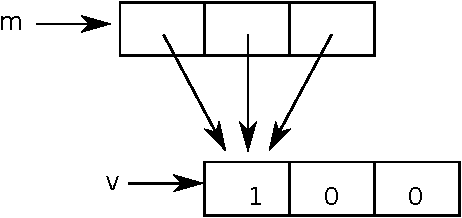
\includegraphics[width=\textwidth]
{img/modification_of_shared_elements_of_a_vector}}
	\caption{Представление в памяти вектора с разделением элементов}
	\label{fig:modification_of_shared_elements_of_a_vector}
\end{figure}

Если значение инициализации вектора (второй аргумент функции
\texttt{Array.create}) простое, атомарное, то оно копируется каждый раз и
совместно используется если это значение структурное.

Мы называем атомарным значением то, размер которого не превышает стандартный
размер значений Objective CAML, то есть \texttt{memory word} --- целое, символ,
булевый и конструкторы констант. Другие значения, называемые структурные,
представлены указателем на зону памяти. Эта разница объяснена более детально в
главе \ref{??}.

Векторы чисел с плавающей запятой есть особый случай. Несмотря на то что эти
числа (\texttt{float}) --- структурные значения, при создании вектора начальное
значение копируется. Делается это для оптимизации. В главе \ref{??}, в которой
обсуждается интерфейс с языком C мы обсудим эту проблему.

\subsubsection{Не квадратная матрица}

Матрица, вектор векторов, не обязательно должна быть квадратной. Действительно,
мы можем заменить вектор на другой вектор с иным размером, что удобно для
ограничения размера матрицы. Следующее значение \texttt{t} создаёт треугольную
матрицу для коэффициентов треугольника Паскаля.

\begin{lstlisting}[language=OCaml]
# let t = [|
           [|1|];
           [|1; 1|];
           [|1; 2; 1|];
           [|1; 3; 3; 1|];
           [|1; 4; 6; 4; 1|];
           [|1; 5; 10; 10; 5; 1|]
         |] ;;
val t : int array array =
  [|[|1|]; [|1; 1|]; [|1; 2; 1|]; [|1; 3; 3; 1|]; [|1; 4; 6; 4; 1|];
    [|1; 5; 10; 10; 5; 1|]|]
# t.(3) ;;
- : int array = [|1; 3; 3; 1|]
\end{lstlisting}

В этом примере элемент вектора \texttt{t} по индексу \texttt{i} есть вектор
целых чисел размером \texttt{i + 1}. Для манипуляции такой матрицей необходимо
знать размер каждого элемента вектора.

\subsubsection{Копия векторов}

При копировании вектора или конкатенации двух векторов мы получаем новый вектор.
Модификация исходных векторов не повлияет на значение копий, кроме случая
разделения значений рассмотренного ранее.

\begin{lstlisting}[language=OCaml]
# let v2 = Array.copy v ;;
val v2 : int array = [|1; 0; 0|]
# let m2 = Array.copy m ;;
val m2 : int array array = [|[|1; 0; 0|]; [|1; 0; 0|]; [|1; 0; 0|]|]
# v.(1)<- 352;;
- : unit = ()
# v2;;
- : int array = [|1; 0; 0|]
# m2 ;;
- : int array array = [|[|1; 352; 0|]; [|1; 352; 0|]; [|1; 352; 0|]|]
\end{lstlisting}

В приведённом примере видно что копия m содержит лишь указатели на \texttt{v},
если один из элементов \texttt{v} изменён, то \texttt{m2} тоже будет изменён.
Конкатенация создаёт новый вектор длина которого равна сумме длин двух других.

\begin{lstlisting}[language=OCaml]
# let mm = Array.append m m ;;
val mm : int array array =
  [|[|1; 352; 0|]; [|1; 352; 0|]; [|1; 352; 0|]; [|1; 352; 0|];
    [|1; 352; 0|]; [|1; 352; 0|]|]
# Array.length mm ;;
- : int = 6
# m.(0) <- Array.create 3 0 ;;
- : unit = ()
# m ;;
- : int array array = [|[|0; 0; 0|]; [|1; 352; 0|]; [|1; 352; 0|]|]
# mm ;;
- : int array array =
[|[|1; 352; 0|]; [|1; 352; 0|]; [|1; 352; 0|]; [|1; 352; 0|]; [|1; 352; 0|];
  [|1; 352; 0|]|]
\end{lstlisting}

Однако, изменение \texttt{v}, разделяемого \texttt{m} и \texttt{mm}, приведёт к
изменению обоих матриц:

\begin{lstlisting}[language=OCaml]
# v.(1) <- 18 ;;
- : unit = ()
# mm;;
- : int array array =
[|[|1; 18; 0|]; [|1; 18; 0|]; [|1; 18; 0|]; [|1; 18; 0|]; [|1; 18; 0|];
  [|1; 18; 0|]|]
\end{lstlisting}

\subsection{Строки}

Строки можно рассматривать как частный случай массива символов. Однако, по
причинам использования памяти этот тип специализирован и синтаксис доступа к
элементам изменён.

Синтаксис

\begin{lstlisting}[language=OCaml]
expr1 . [expr2]
\end{lstlisting}

Элементы строки могут быть физически изменены.

Синтаксис

\begin{lstlisting}[language=OCaml]
expr1 . [expr2] <- expr3
\end{lstlisting}

\begin{lstlisting}[language=OCaml]
# let s = "hello";;
val s : string = "hello"
# s.[2];;
- : char = 'l'
# s.[2]<-'Z';;
- : unit = ()
# s;;
- : string = "heZlo"
\end{lstlisting}

\subsection{Изменяемые поля записей}

Поля записи могут быть объявлены изменяемыми. Для этого достаточно указать при
декларации типа поля ключевое слово \texttt{mutable}

Синтаксис

\begin{lstlisting}[language=OCaml]
type name = { ...; mutable name : t ; ...}
\end{lstlisting}

Пример определения точки плоскости.

\begin{lstlisting}[language=OCaml]
# type point = { mutable xc : float; mutable yc : float } ;;
type point = { mutable xc : float; mutable yc : float; }
# let p = { xc = 1.0; yc = 0.0 } ;;
val p : point = {xc = 1.; yc = 0.}
\end{lstlisting}

Для изменения значение поля объявленного \texttt{mutable} используйте следующий
синтаксис.

Синтаксис

\begin{lstlisting}[language=OCaml]
expr1.nom <- expr2
\end{lstlisting}

Выражение \texttt{expr1} должно быть типа запись содержащее поле \texttt{nom}.
Операция модификации возвращает значение типа \texttt{unit}.

\begin{lstlisting}[language=OCaml]
# p.xc <- 3.0 ;;
- : unit = ()
# p ;;
- : point = {xc = 3.; yc = 0.}
\end{lstlisting}

Напишем функцию перемещения точки, которая изменяет её координаты. Здесь мы
используем локальную декларацию с фильтражом, для упорядочения побочных
эффектов.

\begin{lstlisting}[language=OCaml]
# let moveto p dx dy =
   let () = p.xc <- p.xc +. dx
   in p.yc <- p.yc +. dy ;;
val moveto : point -> float -> float -> unit = <fun>
# moveto p 1.1 2.2 ;;
- : unit = ()
# p ;;
- : point = {xc = 4.1; yc = 2.2}
\end{lstlisting}

Мы можем определить изменяемые или не изменяемые поля, только поля, помеченные
ключевым словом \texttt{mutable}, будут изменяемые.

\begin{lstlisting}[language=OCaml]
# type t = { c1 : int; mutable c2 : int } ;;
type t = { c1 : int; mutable c2 : int; }
# let r = { c1 = 0; c2 = 0 } ;;
val r : t = {c1 = 0; c2 = 0}
# r.c1 <- 1 ;;
Error: The record field label c1 is not mutable
# r.c2 <- 1 ;;
- : unit = ()
# r ;;
- : t = {c1 = 0; c2 = 1}
\end{lstlisting}

Далее, мы приводим пример использование записей с изменяемыми полями и массивов
для того чтобы реализовать структуру стека (см \ref{??}).

\subsection{Указатели}

Objective CAML предлагает полиморфный тип \texttt{ref}, рассматриваемый как
указатель на любое значение. В Objective CAML указатель точнее будет назвать
указатель на значение. Указываемое значение может быть изменено. Тип
\texttt{ref} определён как запись с изменяемым полем.

\begin{lstlisting}[language=OCaml]
type 'a ref = {mutable contents:'a}
\end{lstlisting}

Создать ссылку на значение можно функцией \texttt{ref}. Указываемое значение
может быть получено использованием префикса !. Для модификации значения
используем инфиксную функцию (:=).

\begin{lstlisting}[language=OCaml]
# let x = ref 3 ;;
val x : int ref = {contents = 3}
# x ;;
- : int ref = {contents = 3}
# !x ;;
- : int = 3
# x := 4 ;;
- : unit = ()
# !x ;;
- : int = 4
# x := !x+1 ;;
- : unit = ()
# !x ;;
- : int = 5
\end{lstlisting}

\subsection{Полиморфизм и изменяемые значения}

Тип \texttt{ref} параметризованный (\ref{sec:parametrized_types}), что позволяет
создавать указатели на любой тип. Однако, существует несколько ограничений.
Представим, что нет никаких ограничений и мы можем объявить

\begin{lstlisting}[language=OCaml]
let x = ref [] ;;
\end{lstlisting}

В этом случае тип переменной \texttt{х} будет \texttt{'a list ref} и можем
изменить значение способом не соответствующим статической типизации Objective
CAML.

\begin{lstlisting}[language=OCaml]
x := 1 :: !x ;; x := true :: !x ;;
\end{lstlisting}

При этом получаем одну и ту же переменную типа \texttt{int list} в один момент и
\texttt{bool list} в другой.

Во избежании подобной ситуации, система типов Objective CAML использует новую
категорию типа переменной --- слабо типизированные переменные. Синтаксически,
они отличаются предшествующим символом подчёркивания.

\begin{lstlisting}[language=OCaml]
# let x = ref [] ;;
val x : '_a list ref = {contents = []}
\end{lstlisting}

Переменная типа \texttt{'\_a} не является параметром типа, то есть её тип не
известен до момента её реализации. Лишь в момент первого использования
\texttt{x}, после объявления, тип будет окончательно зафиксирован.

\begin{lstlisting}[language=OCaml]
# x := 0::!x ;;
- : unit = ()
# x ;;
- : int list ref = {contents = [0]}
\end{lstlisting}

Таким образом тип переменной \texttt{x int list ref}.

Тип, содержащий неизвестную, является мономорфным, не смотря на то что его тип
ещё не был указан и невозможно реализовать то что неизвестно полиморфным типом.

\begin{lstlisting}[language=OCaml]
# let x = ref [] ;;
val x : '_a list ref = {contents = []}
# x := (function y -> ())::!x ;;
- : unit = ()
# x ;;
- : ('_a -> unit) list ref = {contents = [<fun>]}
\end{lstlisting}

В этом примере, не смотря на то что мы реализуем неизвестную типом a priori
полиморфным (\texttt{'a->unit}), тип остался мономорфным с новой неизвестной
типа.

Это ограничение полиморфизма распространяется не только на указатели, но и на
любое значение содержащее изменяемую часть: массивы, записи с полями объявленные
\texttt{mutable}, и так далее. Все параметры типа, даже не имеющие никакого
отношения к модифицируемым атрибутам, есть переменные слабого (\texttt{weak})
типа.

\begin{lstlisting}[language=OCaml]
# type ('a,'b) t = { ch1 :'a list ; mutable ch2 : 'b list } ;;
type ('a, 'b) t = { ch1 : 'a list; mutable ch2 : 'b list; }
# let x = { ch1 = [] ; ch2 = [] } ;;
val x : ('a, '_b) t = {ch1 = []; ch2 = []}
\end{lstlisting}

{\it Предупреждение}


Эта модификация типа повлияет на чисто функциональные программы.
Если к полиморфной переменной применена полиморфная функция, то в результате мы
получим переменную слабого типа, так как нельзя не учитывать что функция может
создать физически изменяемое значение. Иными словами, результат будет всегда
мономорфный.

\begin{lstlisting}[language=OCaml]
# (function x -> x) []  ;;
- : 'a list = []
\end{lstlisting}

Тот же результат мы получим для частичных функций.

\begin{lstlisting}[language=OCaml]
# let f a b = a ;;
val f : 'a -> 'b -> 'a = <fun>
# let g = f 1 ;;
val g : '_a -> int = <fun>
\end{lstlisting}

Для получения полиморфного типа необходимо вычесть второй аргумент \texttt{f} и
применить её:

\begin{lstlisting}[language=OCaml]
# let h x = f 1 x ;;
val h : 'a -> int = <fun>
\end{lstlisting}

Действительно, выражения определяющее \texttt{x} есть функциональное выражение
\texttt{function x -> f 1 x}. Его вычисление даст замыкание, которое не рискует
произвести побочный эффект, так как тело функции не вычислено.

В общем случае мы делаем различие между т.н. \enq{не расширяемыми} выражениями,
которые не вызывают побочных эффектов при вычислении и между \enq{расширяемыми}
выражениями. Система типов Objective CAML классифицирует выражения в
соответствии с синтаксисом:

\begin{itemize}
	\item выражения не расширяемые состоят в основном из переменных,
конструкторов не изменяемых значений и абстракций

	\item расширяемые выражения включают в себя преимущественно создание и
применение изменяемых значений. Сюда также необходимо включить такие структуры
управления как условные операторы и сопоставление с образцом.
\end{itemize}
